\documentclass{beamer}
%% Possible paper sizes: a0, a0b, a1, a2, a3, a4.
%% Possible orientations: portrait, landscape
%% Font sizes can be changed using the scale option.
\usepackage[size=a0,orientation=landscape,scale=1.6]{beamerposter}
\usetheme{LLT-poster}
\usecolortheme{ComingClean}
\newcommand{\columnWidth}{.315}
% \usecolortheme{Entrepreneur}
% \usecolortheme{ConspiciousCreep}  %% VERY garish.

\usepackage[utf8]{inputenc}
\usepackage[T1]{fontenc}
\usepackage{libertine}
\usepackage[scaled=0.92]{inconsolata}
\usepackage[libertine]{newtxmath}

\author[uni@email-master.de]{Jan Sieber}
\title{Image Completion}
\institute{Ruprecht-Karls-University Heidelberg}
% Optional foot image
\footimage{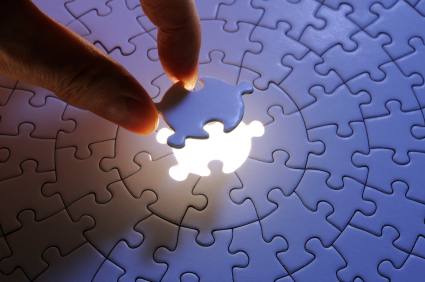
\includegraphics[width=0.08\textwidth]{completion_puzzle.jpg}}

\begin{document}
\begin{frame}[fragile]\centering

\begin{columns}[T]

%%%% First Column
\begin{column}{\columnWidth\textwidth}

\begin{block}{Overview}
    \begin{itemize}
	\item Fill occluded image with suitable data.\\
      \begin{center}
          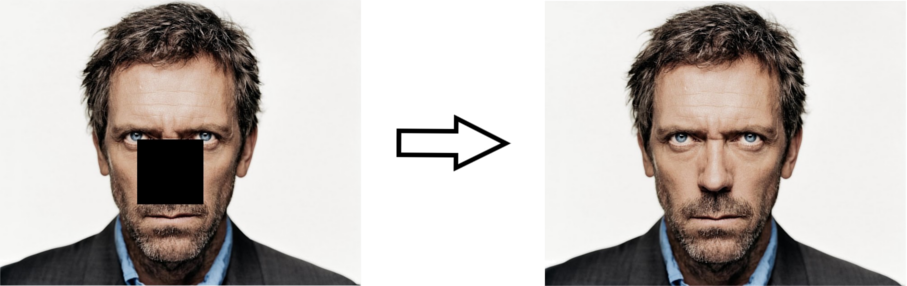
\includegraphics[width=.60\textwidth]{sample_new.png}
      \end{center}
      \begin{itemize}
        \item Image Stitching\\
        $\implies$ Find best image. Copy \& paste occluded parts.
        \item Variational Autoencoder \\
        $\implies$ Make VAE generate image. Copy \& paste occluded parts.
        \item Deep Feature Interpolation\\
        $\implies$ Manipulate occluded image in feature space. Reconstruct image from vector.
      \end{itemize}
    \end{itemize}
\end{block}


\begin{block}{Feature Extraction}
  \begin{itemize}
    \item VGG-19 \\
    \begin{center}
        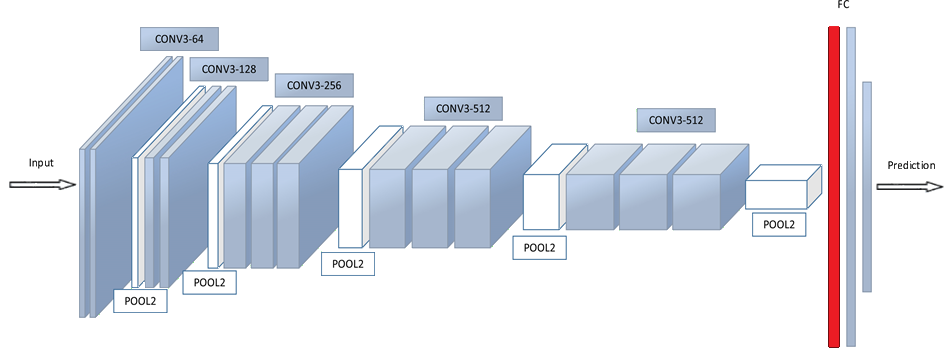
\includegraphics[width=.70\textwidth]{VGG19.png}
    \end{center}
    \item Pre-trained on ILSVRC-14
      \begin{itemize}
      	\item Object recognition/classification contest with 200 object categories
      \end{itemize}
  \end{itemize}
\end{block}

\begin{block}{Image Stitching}
\begin{itemize}
	\item Find the best image
    \begin{itemize}
        \item 100 nearest neighbor search
        \item Filter again with pixel and landmark loss
    \end{itemize}
	\item Find transformation according to landmarks
    \item Fill occluded parts with transformed image
\end{itemize}
$\implies$ Generalizes to data with labels due to nearest neighbor search
\end{block}

\end{column}

%%%% Second Column
\begin{column}{\columnWidth\textwidth}

\begin{block}{Variational Autoencoder}
\begin{itemize}
   \item Train VAE on not occluded images
   \item Generate image and stitch it\\
  $\implies$ No label specific generation possible
  \\ \ \\
  \item Add label vector to intermediate vector for decoder while training \\
  \begin{itemize}
    \item Decoder learns $p(X|z,c)$ instead of $p(X|z)$
    \item C can be the softmax output of classification network
  \end{itemize}
  \begin{center}
      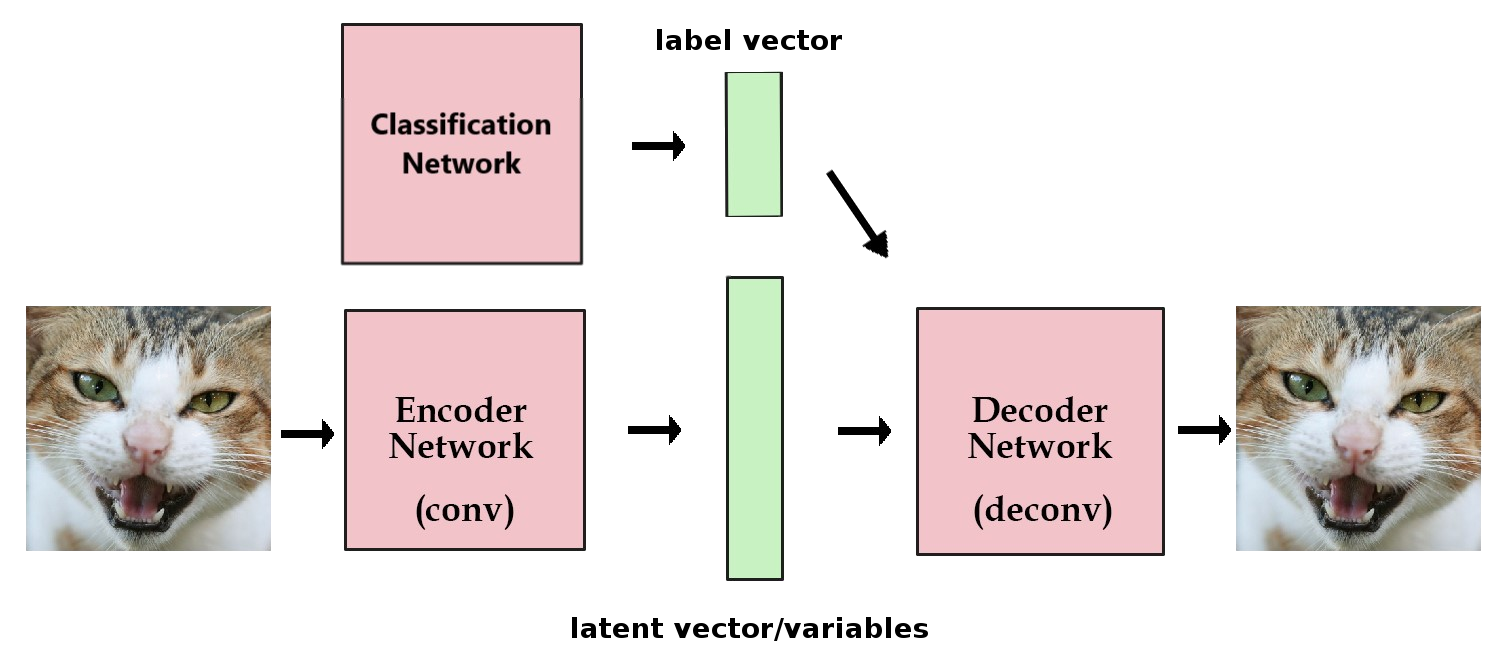
\includegraphics[width=.90\textwidth]{autoenc2.png}
  \end{center}
  $\implies$ Label specific generation possible
  \\ \ \\
  \item Encoder (LFW)\\
  \begin{center}
      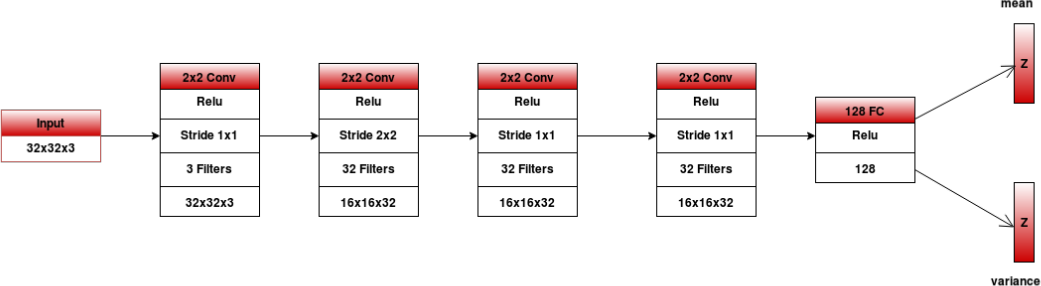
\includegraphics[width=.90\textwidth]{cifar10_encoder.png}
  \end{center}
      \item Decoder (LFW)\\
      \begin{center}
          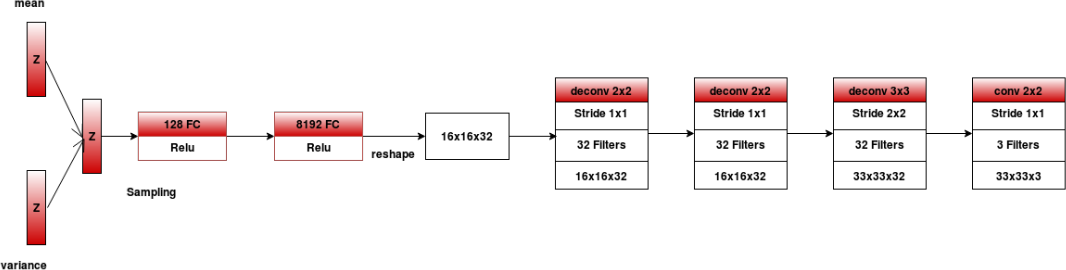
\includegraphics[width=.90\textwidth]{cifar10_decoder.png}
      \end{center}
\end{itemize}
\end{block}
\end{column}
%%%% Third Column
\begin{column}{\columnWidth\textwidth}


\begin{block}{Deep Feature Interpolation}
\begin{center}
	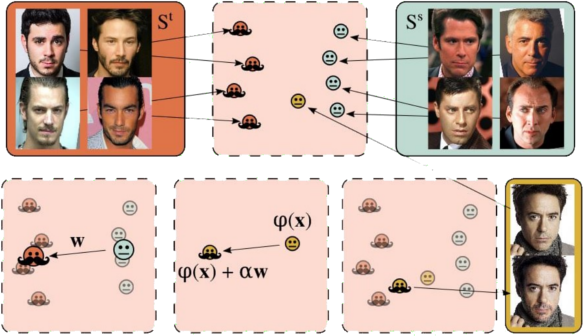
\includegraphics[width=.8\textwidth]{dfi.PNG}
\end{center}
\begin{itemize}
	\item Trying to complete occluded image $I_1$
	\item Get feature vector $\sigma (I_1)$ of $I_1$
	\item Two datasets
    \begin{itemize}
        \item Occluded images $D_1$ \textbf{and} not occluded images $D_2$
    \end{itemize}
    \item Find 100 nearest neighbors in both datasets according to feature vector
    \item Get the difference vector
    \begin{align*}
    	diff = \frac{1}{100} \sum_{x \in F_{2}} \sigma(x) - \frac{1}{100} \sum_{x \in F_{1}} \sigma(x)
    \end{align*}
    \item Add scaled diff to feature vector of $I_1$
    \begin{align*}
    	target = \sigma (I_1) + \alpha \cdot diff
    \end{align*}
    \item Reconstruct the image according to manipulated feature vector by inversion of neural network
    \begin{itemize}
        \item Forward pass image \\
        $\implies$ First forwardpass is black image
        \item Compute loss
        \begin{align*}
            L &= \frac{1}{2} ||target - \sigma_{black}||_2^2 + \lambda R_V\\
            R_V &= \sum_{i,j} ((\sigma_{black_{i,j+1}} - \sigma_{black_{i,j}})^2 + (\sigma_{black_{i+1,j}} - 						\sigma_{black_{i,j}})^2)^{\frac{\beta}{2}}
        \end{align*}
        \item Get gradients w.r.t input image
        \item Manipulate pixels according to gradients
    \end{itemize}
\end{itemize}



\end{block}
\end{column}

\end{columns}


\addtobeamertemplate{block begin}{%
  \setlength{\textwidth}{0.986\textwidth}%
}{}
\begin{block}{Results}
 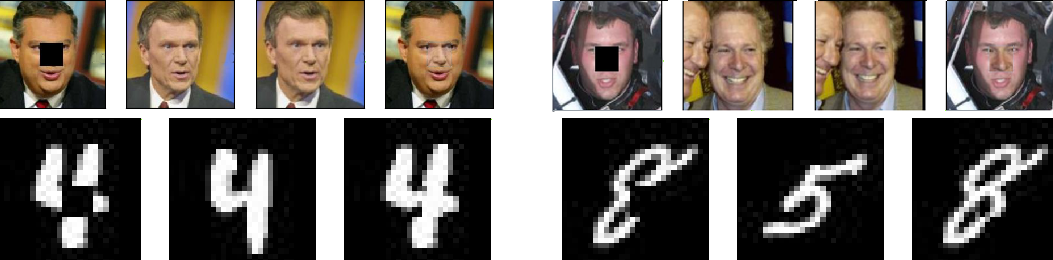
\includegraphics[width=.3\textwidth]{results/stitching_final2.png}
 \hskip6.0ex
 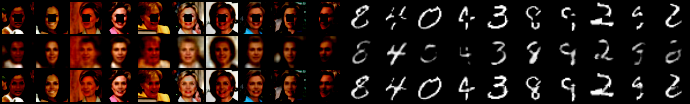
\includegraphics[width=.49\textwidth]{results/VAE-final.png}
 \hskip6.0ex
 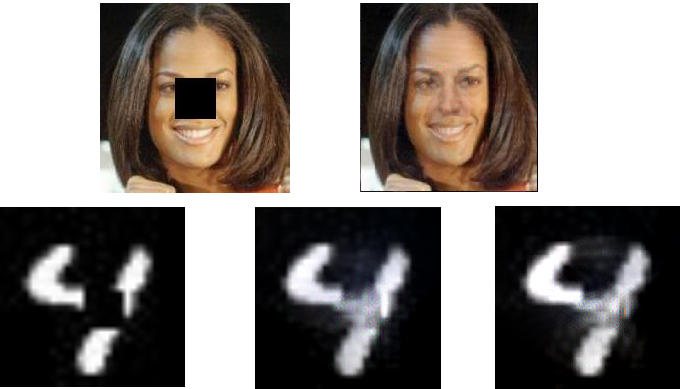
\includegraphics[width=.13\textwidth]{results/DFI-final2.png}
\end{block}
\hskip10.0ex



\end{frame}
\end{document}